\documentclass{book}
\usepackage[ngerman]{babel}
\usepackage{tcolorbox}
\usepackage{amssymb}
\usepackage{fancyvrb}
\usepackage{graphicx}
\graphicspath{./images}
\begin{document}
\begin{titlepage}
    \centering
	{\LARGE \textsc{Hochschule Darmstadt}\par}
	\vspace{1cm}
	{\Large \textsc{Zusammenfassung: 1. Semester}\par}
	\vspace{1.5cm}
	{\huge\bfseries Algorithmen und Datenstrukturen\par}
	\vspace{2cm}
	{\Large\itshape Leonhard Breuer\par}

% Bottom of the page
	{\large \today\par}
\end{titlepage}
\tableofcontents

\chapter{Der Begriff Algorithmus}
\paragraph{Den Begriff Algorithmus} gibt es bereits seit dem Mittelalter.
\paragraph{Das Konzept Algorithmus} war bereits den alten Griechen bekannt.

\section{Sieb des Erasthostenes}
Das S.d.E. ermöglicht das Finden aller Primzahlen bis zu einer gewählten maximalen Zahl $n$.
\paragraph*{Ablauf des Algorithmus} ist wie folgt
\begin{enumerate}
	\item Schreibe alle Zahlen von 1 bis $n$ auf.
	\item Für alle Zahlen $i$ von 2 bis $\sqrt{n}$: Alle Vielfachen von $i$ streichen.
	\item Schreibe alle nicht gestrichenen Zahlen herraus.
\end{enumerate}
\section{Algorithmus des Euklied (ggT)}
Der Algorthimus des Euklied dient zum Herausfinden des \textit{größten gemeinsamen Teilers} zweier Zahlen.
\paragraph*{Ablauf des Algorithmus} ist wie folgt. \\
Ausgehend von den Zahlen $m$ und $m$ < 0 sowie $r$ welche den Rest der (ganzzahligen) Division repräsentiert.
\begin{enumerate}
	\item Teile $m$ durch $n$ mit Rest $r$ (es ergibt sich $r \geq n$).
	\item Wenn $r = 0$, fertig mit Ergebnis $n$.
	\item Ersetze $m$ mit $n$ und $n$ mit $r$ und mache mit \textit{1.} weiter.
\end{enumerate}
\section{Algorism}
Das Wort \textit{Algorism} beschreibt das Addieren im Stellenwertsystem.
\paragraph*{Ablauf des Algorithmus} ist wie folgt
\begin{enumerate}
	\item Schreibe die zu addierenden Zahlen rechtsbündig untereinenander.
	\item Beginne ganz rechts mit der ersten Zahl.
	\item Addiere die über dem Strich stehenden Ziffern der aktuellen Stelle zusammen.
	\item Schreibe das Ergebnis unter den Strich
	\item Setze diese Operationen für alle restlichen Stellen (beider Zahlen) fort.
\end{enumerate}

\chapter{Graphen und Bäume}
Graphen und Bäume werden in der Informatik oftmals zur Beschreibung und Vereinfachung von  Problemen benötigt.
\paragraph*{Ein Graph} besteht aus \texttt{Knoten (nodes)} und \texttt{Kanten (edges)}.
\subparagraph*{Knoten} bilden die Menge \texttt{V} von Objekten \textit{v}.
\subparagraph*{Kanten} bilden die Menge \texttt{E} von Tupeln \textit{e = (v, w)} mit $v,w \in V$. 
\section{Graphen}
\subsection{Pfade} Man unterscheidet zwischen \texttt{offenen} und \texttt{geschlossenen} Pfaden.
\begin{description}
	\item[offener Pfad] Start- und Endpunkt sind unterschiedlich
	\item[geschlossener Pfad]  Führt am Ende an der Startpunkte zurück (Schleife)
\end{description}
\subsection{Annotationen}
Annotationen können anliegen, an
\begin{itemize}
	\item \texttt{Knoten}: Als Knotengewicht
	\item \texttt{Kanten}: Als Kantengewicht
\end{itemize}
Annotationen, seltener Gewichtungen, ermöglichen es Algorithmen, bzw. den kürzesten Weg zu ermitteln.
\subsection{Grad eines Knotens}
\begin{description}
	\item[Bei gerichteten Kanten] unterscheidet man Aus- und Eingangsgrad.
	\item[Bei ungerichteten Kanten] spricht man nur vom "Grad". 
\end{description}
Vereinfacht stellt der "Grad" eines Knoten die Anzahl der ein-/ausgehenden Verbindungen des Knoten(im Falle eines gerichteten Graphen) 
und der Gesamtanzahl der Verbindungen des Knoten (im Falle eines ungerichteten Graphens) dar.
\subsection{Gerichtete Graphen}
\begin{itemize}
	\item Alle Pfade sind \textit{offen}.
	\item auch \textit{Digraph} oder \textit{directed graph}
\end{itemize}
\subsection{Gewichtete Graphen}
Ein Graph ist gewichtet, sobald er über Annotationen verfügt.
\subsection{Dependenzgraph (DAG)}
Bei einem Dependenzgraphen beschreiben die Kanten, welche Tätigkeiten/Aufgaben vor 
einer anderen erfüllt werden müssen.
Enthält der gerichtete Graph hierbei keine Zyklen, so spricht man vom \textit{directed acyclic graph} oder kurz \textit{DAG}.
\subsection{Ungerichteter Graph / Cliquen}
Eine \textit{ungerichtete} Kante verhält sich wie zwei gerichtete Kanten. (eine hin und eine andere zurück)

\paragraph{Zusammenhang} Wenn von einem Element aus, alle anderen Elemente (Knoten) in einem Graphen erreichbar sind,
dann spricht man von einem zusammenhängenden Graphen. Gruppen, welche zwischen sich verbunden aber nicht mit anderen Gruppen verbunden sind, nennt man \textit{Zusammenhangskomponenten}
\subsection{Multigraph} 
Gibt es mehrere Kanten zwischen zwei Knoten (sowohl gerichtet als auch ungerichtet), so spricht man von einem
Multigraph.
\section{Bäume}
Ein Baum ist \textit{zusammenhängender} \textit{ungerichteter} Graph ohne \textit{geschlossenen} Pfad.
\subsection{Knoten und Blätter}
\begin{description}
	\item[Knoten mit Grad 1]  werden als Blatt (oder engl. Leaf) bezeichnet.
	\item[Andere Knoten] werden als innere Knoten bzw. \textit{inner leaf} bezeichnet. 
	\item[Elter(n)] ist der übergeordnete Knoten
	\item[Kind] ist der untergeordnete Knoten 
\end{description}
\subsection{Bäume - Höhe, Grad}
\begin{description}
	\item[Grad] Der Grad eines Baumes ist immer der höchste Grad eines Knotens.
	\item[Höhe] maximale Pfadlänge
\end{description}
\section{Kontrollstrukturen}
\begin{description}
	\item[Sequenz] Dinge nacheinander ausführen.
	\item[Alternative] Bedingte Befehlsausführung (if/else; switch; ternary)
	\item[Schleifen] (do/while; while; for)   
	\item[Funktionen]
	\item[Sprünge] nicht verwendet (goto) 
\end{description}

\chapter{Felder und Strings}
\section{Felder}
\begin{itemize}
	\item feststehender Datentyp
	\item konstankte Größe
\end{itemize}
\subsection{Speicherung}
Einträge in Felder werden immer nur im jeweiligen Datentyp gemacht. Die Größe eines Arrays beträgt also immer
$$size_{array} = count \times size_{data\_type}$$
\subsection{Namenskonventionen}
\begin{description}
	\item[i] repräsentiert den Index (bei mehreren Schleifen ineinander auch \textit{j} oder \textit{k})
	\item[n] repräsentiert die Größe (selten auch \textit{m}, \textit{n1} oder \textit{n2})  
\end{description}
\subsection{Array vs. Vector}
Während bei einem \textit{Array} die Größe bereits zur Compiletime feststehen muss,
kann die Größe eines \textit{Vectors} auch noch zur Runtime geändert werden.
\subsection{Mehrdimensionale Felder}
Ein mehrdimensionales Feld enthält mehrere (meist eindimensionale) Felder.
\section{Strings}
\begin{description}
	\item[ASCII] \textit{(American Standard Code for Information Interchange)} 32-127 Zeichen (7bit)
	\item[ISO-8859]  enthält alle \textit{ASCII}-Zeichen (0-127) und weitere Zeichen (128-256) anderer Sprachen.
	\item[UTF-8] enthält alle \textit{ASCII}-Zeichen (0-127) und weitere Zeichen (128 - ...) anderer Sprachen.
\end{description}
\subsection{Besonderheit von UTF-8}
Die Besonderheit von \textit{UTF-8} gegenüber \textit{ISO-8859} liegt in der variablen Speicherlänge der einzelnen Zeichen.
Die meisten Zeichen (des normalen Alphabets) besitzen eine Speicherlänge von einem Bit. Besondere Zeichen wie die deutschen Umlaute (\textit{ä, ü, ö}) besitzen eine Speicherlänge
von 2 Bit.
\begin{tcolorbox}
	UTF-8 ermöglicht es einem Zeichen eine Länge von 1 - 4 bit zu haben.
\end{tcolorbox}
\subsection{Nutzung in C++}
\paragraph{char*} einfach…
\begin{itemize}
	\item Zeichenkette solange bis eine \textit{0} kommt.
	\item Pro String nur ein Byte.
	\item beliebige Länge
	\item Die meisten Betriebssysteme liefern Strings/Werte in diesem Format.
\end{itemize} 
… aber echt unpraktisch.
\paragraph{std::string} \textit{std::string} bietet eine Speicherkapselung, was die manuelle Speicherverwaltung
überflüssig macht. 
\begin{itemize}
	\item Implementierung abhängig von der Laufzeitumgebung.
	\item Häufig: Angelegt auf Heap -> Adresse durch Variable gehalten. 
\end{itemize}
\begin{tcolorbox}
	\begin{itemize}
		\item sizeof(int) = 4
		\item sizeof(std::string) = 32
	\end{itemize}
	Der String ermöglicht also Zeichenketten von ca. 32 Zeichen ohne zusätzlichen Platz auf dem Heap.
\end{tcolorbox}
\chapter{Iteration und Rekursion}
\paragraph{Iteration} bezieht sich auf die Wiederholung durch Aneinanderreihung mithilfe von Schleifen.
\paragraph{Rekursion} bezieht sich auf die Wiederholung durch Ineinanderschachtelung mithilfe von Funktionen.
\begin{tcolorbox}
	\textbf{Beispiel}
	\begin{description}
		\item [Iteration] mit einer for-Schleife
	
	\begin{verbatim}
		void f1(int n, int m){
			for (int i=n; i<=m; i++){
				cout << i << endl;
			}
		}
	\end{verbatim}
	\item[Rekursion] mit einer Funktion
	\begin{verbatim}
		void f6 (int n, int m){
		if (m<n) return;
		f6(n,m-1);
		cout << m << endl;
		}
	\end{verbatim}
\end{description}
\end{tcolorbox}
Es gibt hier kein klares besseres Element. Beide haben ihre Daseinsberechtigung. 
Eine "bessere" Lösung mit einem der beiden Arten ist immer von dem vorliegenden Problem abhängig.
\chapter{O-Notation}
\section{Union-Find}
Der Union-Find Algorithmus ist ein äußerst vielseitiger Algorithmus.
\subsection{Anwendungsbeispiele}
\begin{itemize}
	\item Pixel auf einem Foto
	\item Freunde in Sozialen Netzwerken
	\item Computer in einem Netzwerk
	\item Elemente in einer mathematischen Menge
\end{itemize}
\subsection{Funktionen}
\paragraph{find} Diese Funktion prüft, ob sich zwei Elemente in der selben Zusammenhangskomponente befinden bzw. es einen Weg von der einen zur anderen gibt.
\paragraph{unify} Diese Funktion ersetzt die Komponenten zweier Elemente mit ihrer Vereinigungsmenge bzw. verknüpgt zwei Elemente.
\subsection{Abwandlungen des Union-Find}
\paragraph{Quick-Find}
\subparagraph*{Basis} Die Basis für den \textit{Quick-Find} macht ein Feld \textbf{id[]} mit Größe \textit{n} und Datentypen \textit{int}. Zwei Objekte sind dann verbunden, wenn sie diesselbe ID haben.
\subparagraph*{Geschwindigkeit} Man stellt fest, dass der Quick-Find-Algorithmus zulangsam ist.
\newline
\begin{center}
\begin{tabular}{|c|c|c|c|}
	\hline
	\textbf{Algorithmus} & \textbf{init} & \textbf{unify} & \textbf{find}  \\
	\hline
	Quick-Find & N & N & 1 \\
	\hline
\end{tabular}
\end{center}
Die \textit{unify}-Operation vom Quick-Find ist zu langsam. Da die Laufzeit bei N Objekten \textbf{$N^{2}$} beträgt.
\paragraph{Quick-Union}
\subparagraph*{Basis} Die Basis ist identisch zum \textit{Quick-Find}. id[i] ist \textit{Elter} von i - Wurzel i ist $id[id[id[...id[i]...]]]$.
\subparagraph*{Geschwindigkeit} Auch der Quick-Union hat keine großen Vorteile im Vergleich zum Quick-Union, auch wenn er häufig schneller ist.
\begin{center}
	\begin{tabular}{|c|c|c|c|}
		\hline
		\textbf{Algorithmus} & \textbf{init} & \textbf{unify} & \textbf{find}  \\
		\hline
		Quick-Find & N & N (inkl. Wurzel suche) & N \\
		\hline
	\end{tabular}
	\end{center}
\paragraph{Weighted Quick Union} Ein Problem des Quick Union waren die zu groß werdenden Bäume. 
Dies soll mit dem Gewichten verbessert werden. 

\subparagraph*{Geschwindigkeit} Die Geschwindigkeit des Weighted Quick Union 
ist deutlich besser als die beiden anderen Implementierungen.

\begin{center}
	\begin{tabular}{|c|c|c|c|}
		\hline
		\textbf{Algorithmus} & \textbf{init} & \textbf{unify} & \textbf{find}  \\
		\hline
		Weighted Quick Union & N & ld N (inkl. Wurzel suche) & ld N \\
		\hline
	\end{tabular}
	\end{center}

\paragraph{Quick-Union mit Pfadkompression}
\subparagraph*{Basis/Idee} Nach dem Fund der Wurzel, werden alle besuchten Knoten direkt an die Wurzel angehängt.
\subparagraph*{Geschwindigkeit} Die Auswertung der Laufzeitkomplexität von Weighted Quick Union mit Pfadkompression ist zu kompliziert.
Laut Hopcraft-Ulman und Tarjan benötigt man \textbf{M} Union-Find-Operationen auf \textbf{N}-Elemente weniger als c(N + M $\times$ N) Feldzugriffe.
Das führt zu einer beinahe linearen Laufzeitkomplexität.

\subsection{Zusammenfassung Union-Find-Algorithmen}
Die Algorithmen folgende Laufzeitkomplexität (im Worst Case) auf:
\begin{center}
\begin{tabular}{|c|c|}
	\hline
	\textbf{Algorithmus} & \textbf{Laufzeitkomplexität (Worst Case)} \\
	\hline
	Quick Find & M $\times$ N \\
	Quick Union & M $\times$ N \\
	Weighted Quick Union & N + M $\times$ $log$ N \\
	Quick Union (Pfadkompression) & N + M $\times$ $log$ N \\
	Weigthed Quick Union (Pfadkompression) & N + M $\times$ $ld$ N \\
	\hline
\end{tabular}
\end{center}
\section{Skalierung quadratischer Probleme}
Die Skalierung von Quadratischen Problemen ist sehr schwer. 
Mit stetiger Evolution von Computer steigen auch die Anforderungen an diese.
Die zu lösenden Problematiken werden immer größer, komplexer und somit letztendlich auch rechenaufwendiger.\\
Die einzige Lösung für diese Problematik: 
\begin{center}
	\textit{Effizientere Algorithmen}
\end{center}
\section{Komplexitätstheorie}
Die zentrale Frage der Komplexitätstheorie lautet
$$P = NP$$

\begin{description}
	\item[P] Klasse von Problemen, die praktisch lösbar sind. (deterministisch \& polynomiell)
	\item[NP] Klasse von Problemen, die praktisch überprüfbar sind. (nicht deterministisch \& polynomiell)
\end{description}

\subsection{O-Notation}
Die \textit{O-Notation} beschreibt das Verhalten von Algorithmen in Richtung unendlich. \\
O(g(n)) ist eine Menge, die alle FUnktionen enthält, die unendlich von g durch Multiplikation mit einer Konstanten \textit{c} übertrumpft werden.
\paragraph{Einige Rechenregeln mit der O-Notation}
\begin{itemize}
	\item $f(n) = O(f(n))$
	\item $O(c \times f(n)) = O(f(n))$
	\item $O(f(n)) + O(g(n)) = O(\max(f(n), g(n)))$
	\item $O(f(n)) \times O(g(n)) = O(f(n) \times g(n))$
	\item $f(n) \times O(g(n)) = O(f(n) \times g(n))$
\end{itemize}
\paragraph{Addition}
Bei der Addition der O-Notation (dem Ausführen einer Aufgabe vor einer anderen) spielt nur die komplexere Aufgabe eine Rolle.
Beispiel: \\
$O(log N) + O(N) = O(N)$\\
$O(N) + O(N^{2}) = O(N^{2})$

\paragraph{Multiplizieren}
Im Gegensatz zum Addieren, erhöht die Multiplikation die Gesamtkomplexität.
\begin{tcolorbox}
	Das lässt sich sehr einfach am Beispiel einer Schleife darstellen.
Der Schleifenkörper hat eine Komplexität $O(g(n))$ und wird $f(n)$-Mal ausgeführt.
Das erhöt den Gesamtaufwand zum Produkt $O(g(n) \dot f(n))$
\begin{Verbatim}
for (i = 0; i < n; i++) {
	for (j = 0; j < n; j++) {
		… irgendeine Operation mit O(1) …
	}
}
\end{Verbatim}
\begin{itemize}
	\item Der Schleifenkörper der inneren Schleife wird n mal ausgeführt: $n \dot O(1) = O(n)$
	\item Der Schleifenkörper der äußeren Schleife wird n mal ausgeführt: $n \dot O(n) = O(n \dot n) = O(n^{2})$
\end{itemize}
\end{tcolorbox}

\paragraph{Limitierungen} Die getroffenen Entscheidungen und darausfolgenden Vereinfachungen haben jedoch einige Nachteile:
\begin{itemize}
	\item Algorithmen gleicher Komplexitätsklasse sind nicht unbedingt gleich schnell.
	\item Ein Algorithmus der in der Theorie schneller ist, muss nicht in der Praxis gleichschnell sein.
\end{itemize}

\chapter{Liste, Heap, Stack und Queue}
\section{Liste}
Listen finden sich überall im täglichen Leben.
\subsection{Liste als Datenstruktur}
Es gibt mehrere Möglichkeiten zur Verwaltung von Listen
\begin{itemize}
	\item In einem Array oder \textit{vector}
	\item Als verkettete Liste
\end{itemize}

\subsection{Liste als Array} 
Vorteile:
\begin{itemize}
	\item Einfach zu Implementierungen
	\item Zugriff auf n-tes Element mit O(1)
	\item Prüfung leerer Liste O(1)
	\item Einfügen und Löschen am Ende O(1)
\end{itemize}
Nachteile: 
\begin{itemize}
	\item Einfügen am Anfang und zwischendrin: O(N)
	\item Löschen am Anfang und zwischendrin aufwändig O(N)
	\item Maximaler Platz muss bekannt sein, Speicherschwendung. (Abhilfe durch Vector)
\end{itemize}
\subsection{Liste als verkettete Liste}
Eine verkettete Liste besteht aus der Information selbst und einem Zeiger auf das nächste Element in der Liste.\\
Beispielcode: 
\begin{Verbatim}
	struct node {
		string data;
		node* next;
	}
\end{Verbatim}
Das letzte Element der Liste erhält einen $nullptr$ als Zeiger auf das "nächste" Element.
\begin{table}[htbp]
	\centering
	\begin{tabular}{|c|c|c|}
	\hline
	Operation & Als Array & Als verkettete Liste \\
	\hline
	Element einfügen am Anfang & $O(N)$ & $O(1)$ \\
	Element einfügen am Ende & $O(1)$ & $O(N)$ \\
	Element einfügen an $n$-ter Stelle & $O(N)$ & $O(1)$ (Suche: $O(N)$) \\
	Element löschen am Anfang & $O(N)$ & $O(1)$ \\
	Element löschen am Ende & $O(1)$ & $O(N)$ \\
	Element löschen an $n$-ter Stelle & $O(N)$ & $O(1)$ (Suche: $O(N)$) \\
	Element am Anfang & $O(1)$ & $O(1)$ \\
	Element am Ende & $O(1)$ & $O(N)$ \\
	Element an $n$-ter Stelle & $O(1)$ & $O(N)$ \\
	Element (nach Inhalt) suchen & $O(N)$ & $O(N)$ \\
	Element suchen und löschen & $O(N)$ & $O(N)$ \\
	Anzahl der Elemente ermitteln & $O(1)$ & $O(N)$ \\
	Leere Liste erkennen & $O(1)$ & $O(1)$ \\
	Liste vorne anhängen & $O(N+M)$ & $O(M)$ \\
	Liste hinten anhängen & $O(M)$ & $O(N)$ \\
	\hline
	\end{tabular}
	\caption{Vergleich von Operationen zwischen Arrays und verketteten Listen}
	\label{tab:operationen-vergleich}
	\end{table}

\paragraph{doppelt verkette Listen} Das doppelte Verketten (Endzeiger und Zähler) von Listen ermöglicht für fast alle Operationen auf Listen \textbf{O(1)}.

\section{Stack}
Der Stack (Stapel) ist eine Datenstruktur, die dem LIFO (last in, first out) Prinzip folgt.
Beispiel:
Das zuletzt hinzugefügte Element wird als erstes wieder entfernt.

\subsection{Anwendungen}
Stacks werden verwendet um den Programmfluss, Funktionsaufrufe und lokale Variablen effiziernt zu verwalten. z.B. Bei der Rekursion.

\subsection{Operationen}
\begin{description}
	\item[push(x)] legt das Element x auf den Stack.
	\item[x=pop()] holt das oberste Element vom Stack.  
\end{description}
Es gibt aber noch die Methoden \textit{peek}, \textit{top}, welche dem Aufruf von \textit{x=pop(); push(x)}, also dem Herausheben eines Elements, entsprechen.
Häufig kommt noch die Methode \textit{empty} hinzu, welche den Stack auf seinen Inhalt überprüft (Vermeidung von Laufzeitfehlern.)

\subsection{Geschwindigkeit}
Alle Operationen an einem Stack benötigen \textit{O(1)}.

\subsection{Zusammenhang mit Rekursion}
Stapel (Stacks) werden oft in der Informatik verwendet, um den Aufruf von Funktionen und die Verwaltung von lokalen Variablen während der Rekursion zu unterstützen, da die letzte aufgerufene Funktion immer als erste zurückkehrt, 
was dem Last-In-First-Out (LIFO)-Prinzip entspricht. Dies ermöglicht die effiziente Verwaltung von Funktionsaufrufen und Rückgabewerten.

\section{Queue}
Eine Queue (Schlange) folgt dem FIFO (first in, first out) Prinzip.

\subsection{Anwendungen}
Einfache Anwendungen von Queues finden sich in den meisten Algorithmen.
Sie werden häufig als Datenpuffer / Zwischenspeicher verwendet, z.B. wenn die Daten momentan nicht verarbeitet werden können, jedoch zu einem späteren Zeitpunkt in der selben Reihenfolge wieder abgerufen werden müssen.


\subsection{Operationen}
\begin{description}
	\item[enqueue(x)] Hinzufügen zur Queue (auch \textit{push(x)}).
	\item[x = dequeue()] Entnehmen aus der Queue (auch \textit{x = pop()}).   
\end{description}
Auch hier gibt es mehere weitere Operationen, wie z.B. \textit{empty} mit gleicher Funktionsweise wie bei dem Stack. Oder auch \textit{front}, welche das nächste Element liefert, ohne es zu entnehmen.
\subsection{Geschwindigkeit}
Alle Operationen an einer Queue benötigen \textit{O(1)}.

\section{Heap}
Der Heap dient auch als Zwischenspeicher.
\subsection{Anwendungen}
Der Heap wird genutzt um Platz für Daten zu bieten, deren Größe sich zur Laufzeit ändern kann.
\subsection{Operationen}
\begin{description}
	\item[push\_heap(x)] packt ein Element auf den Heap.
	\item[x = pop\_heap()] nimmt ein Element vom Heap. 
\end{description}
\subsection{Geschwindigkeit}
Die Geschwindigkeit der Operationen an einem Heap sind O(log N).

\chapter{Sortier- und Suchalgorithmen}
Das Sortieren stellt eine der ältesten Anwendungen für Computer dar. 

\section{Eigenschaften von Sortieralgorithmen}
Ein Sortieralgorithmus ist …
\begin{description}
	\item[natürlich], wenn eine bereits (fast) sortierte Liste schneller fertig ist, als eine komplett unsortierte.
	\item[stabil], wenn Reihenfolge der Elemente bleibt bei gleichem Schlüsselwert identisch.
	\item[in place / in situ], wenn die Speichergröße konstant bleibt.
	\item[extern], wenn die Daten nicht im Arbeitsspeicher sondern auf Band oder Platte vorliegen. 
\end{description}

\section{Selectionssort}
\subsection{Idee}
\begin{itemize}
	\item größte Karte $\rightarrow$ ganz rechts.
	\item kleinste Karte $\rightarrow$ ganz links.
\end{itemize}
\subsection{Algorithmus}
Der Algorithmus vom \textit{Selectionssort} läuft wie folgt:
\begin{enumerate}
	\item Alle Elemente $\rightarrow$ Array
	\item Kleinste Zahl suchen
	\begin{enumerate}
		\item Merke Zahl ganz links als \textbf{min} und aktuelle Position \textbf{pos}.
		\item Prüfe ob \textbf{pos+1} kleiner als \textbf{min}. Wenn Ja, neue \textbf{min} und \textbf{pos}.
		\item Mache weiter mit \textit{2.a} bis Ende
	\end{enumerate}
	\item Vertausche die Zahl an der Stelle \textbf{pos} mit der ersten Zahl und in den sortierten Bereich.
	\item Mache mit 2 weiter, bis Ende.
\end{enumerate}
\subsection{Funktionsweise}
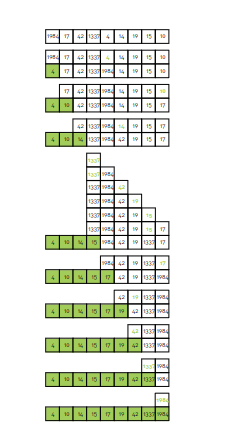
\includegraphics[scale=0.5]{images/selectionssort.png}
\subsection{Eigenschaften}
\begin{description}
	\item[natürlich] ja.
	\item[stabil] ja.
	\item[in place] ja.
\end{description}
\subsection{Laufzeitkomplexität}
\paragraph{Schleifendurchläufe}
Es gibt $(n \dot (n-1))/2$ Schleifendurchläufe
\paragraph{Best-/Worstcase} Bei der \textit{Selectionssort} gibt es keinen Best-/Worstcase, da die innere Schleifen immer durchlaufen wird.
\paragraph{Komplexitätsklasse} Die Komplexitätsklasse des \textit{Selectionssort}-Algorithmus ist
$$O(\frac{(n \dot (n - 1))}{2})$$
$$ = O(\frac{n^{2}-n}{2})$$
$$ = O(n^{2})$$
\section{Insertionsort}
\subsection{Idee}
Bei der Grundidee für den Insertionssort gibt es 2 Varianten:
\begin{itemize}
	\item Nimm nächste Karte $\rightarrow$ in Hand einsortieren von links ein (klein -> groß)
	\item Nimm nächste Karte $\rightarrow$ in Hand einsortieren von rechts ein (groß -> klein) 
\end{itemize}
\subsection{Algorithmus} 
\begin{enumerate}
    \item Zu Beginn umfasst der unsortierte Bereich alle Elemente des Arrays bis auf eines. Das eine Element des sortierten Bereichs ist trivialerweise bereits sortiert.
    \item Sortiere die ganz links stehende Zahl des unsortierten Bereichs in den bereits sortierten Bereich von rechts (große Zahlen) her ein wie folgt:
        \begin{enumerate}
            \item Tausche die neu einzusortierende Zahl immer weiter nach vorne, bis entweder
            \item die Zahl links davon kleiner als die neu einzusortierende Zahl ist – der richtige Platz ist dann gefunden – oder
            \item das Ende erreicht ist – dann ist die neu einzusortierende Zahl die kleinste bisher. (In beiden Fällen wandern dadurch alle Zahlen, die größer als die neu einzusortierende Zahl ist, um eine Position nach rechts.)
        \end{enumerate}
    \item Mache mit Schritt 1 weiter, bis du am Ende bist.
\end{enumerate}

\subsection{Eigenschaften}
\begin{description}
	\item[natürlich] ja
	\item[in place] ja
	\item[stabil] ja  
\end{description}

\subsection{Laufzeitkomplexität}
\paragraph{Schleifenläufe} Hier gibt es maximal $(n \dot (n-1))/2$ Schleifendurchläufe. Ein früheres Ende ist möglich.
\paragraph{Best-/Worstcase} Ja, die innere Schleife wird garnicht durchlaufen. Von $n$ bis $n \dot (n-1) / 2$
\paragraph{Komplexitätsklasse} Hier gibt es mehrere Klassen: \\
Best Case:
$$O(n)$$
Worst Case:
$$O(n^2)$$
\section{TODO}
Andere Sortieralgorithmen hinzufügen.
\section{Binäre Suche}
\subsection{Idee}
Schritt 0: Gehe zur Mitte der Liste
\begin{enumerate}
	\item ist das Element genau dort, fertig.
	\item ist das gesuchte Element kleiner als die Mitte, wiederhole für die vordere Hälfte.
	\item ist das gesuchte Element größer als die Mitte, wiederhole für die hintere Hälfte.
\end{enumerate}
Diese Art zu Suchen, nennt man \textbf{Divide'n'Conquer}.
Nach spätestens \textbf{ld N} haben wir nur noch ein Element.

\end{document}